\documentclass{article}

\usepackage{polski}
\usepackage[utf8]{inputenc}
\usepackage{tikz}
\usepackage{amsmath}
\usepackage{mathtools}
\usepackage{amssymb}

\newcommand{\R}{\mathbb{R}}
\newcommand{\N}{\mathbb{N}}
\newcommand{\Q}{\mathbb{Q}}
\newcommand{\Z}{\mathbb{Z}}
\newcommand{\C}{\mathbb{C}}
\newcommand{\cont}{\mathfrak{c}}
\pagestyle{empty}

\begin{document}
\subsection*{ZAD 2. Sprawdzić przez indukcję, że jeśli $n(r-1)+1$ przedmiotów umieścimy w $n$ szufladach, to pewna szuflada zawiera $\geq r$ przedmiotów}
$1^{\circ}\;n = 1$\smallskip\par
Do jednej szuflady wkładamy $1\cdot(r-1)+1$ przedmiotów, więc w jedynej szufladzie będzie $r$ przedmiotów.\medskip\\
$2^{\circ}$ dla pewnego $n\in\N$ zakładamy, że przy wkładaniu $n(r-1)+1$ przedmiotów do $n$ szuflad w pewnej szufladzie znajdzie się co najmniej $r$ przedmiotów.\smallskip\par
Wówczas, jeśli w $n+1$ szufladach umieścimy $(n+1)(r-1)+1=(n(r-1)+1)+r$ przedmiotów. Czyli do pierwszych $n$ szuflad wkładamy $n(r-1)+1$ przedmiotów, czyli w pewnej będzie ich co najmniej $r$, a do $+1$ szuflady zostanie $r$ przedmiotów.
\newpage
\subsection*{ZAD 3. Pokazać, że wśród 52 liczb całkowitych znajdują się dwie różne, których suma lub różnica dzieli się przez 100.}
  Przy dzieleniu przez 100 możemy mieć resztę bedaca liczba naturalna od 0 do 99 - jest ich 100. Pierwszym 50 resztom (od 0 do 49) możemy przyporzadkować resztę z drugiej połowy, które łącznie sumują się do 100. Dla 50 takim dopełnieniem jest ona sama. \\
  Opiszmy więc 51 szufladek takimi parami. Ponieważ bierzemy 52 liczby całkowite, to na pewno dwie liczby beda należeć do tej samej szufladki - wówczas ich suma (jeśli maja dopełniajace się reszty lub taką sama resztę, ale różne znaki) lub różnica będzie podzielna przez 100.
\newpage
\subsection*{ZAD 4. Dane sa liczby naturalne $1\leq a_1<a_2<...<a_{37}=60$. Wykazać, że $a_j-a_i=13$ dla pewnych $i<j$.}
  Weźmy 13 szufladek i oznaczmy każdą resztą z dzielenia przez 13, czyli liczbą ze zbioru $\{0, 1, 2,..., 12\}$. \\
  Mamy 36 różnych liczb, które rozkladajac do tych szufladek dadzą nam 10 szufladek gdzie jest co najmniej 3 liczby i 3 szufladki, gdzie liczb jest co najmniej 2. Dodatkowo, do szufladki z 8 dojdzie liczba $a_{37}=60$.\\
  Wiemy, że liczba ${60\over13}=4\texttt{ reszty }8$.Tak więc jeśli w 8 szufladkach w których jest co najmniej po 3 liczby mamy tylko takie, ktore skaczą co 26 (np 1, 27, 53), to zostaje co najmniej jedna szufladka, w której liczby muszą znajdować się co najwyżej do liczby 52. Jest ich co najmniej 3, wiec dwie z nich sa oddalone od siebie o dokladnie 13 (gdyz rozpatrujemy 3 różne liczby na przedziale od 1 do 52=13$\cdot$4 dające tę samą reszte przy dzieleniu przez 13).
\newpage
\subsection*{ZAD 5. 41 wież umieszczono na szchownicy 10x10. Pokazać, że można znaleźć 5 wież, które się nie atakują.\\Wskazówka: Wieże atakują po liniach poziomych i pionowych. Zwinąć szachownicę w cylinder łącząc przeciwne strony i pokolorować przekatne 10 kolorami.}
Na poczatku zauważmy, ze skoro wieże atakują się tylko po liniach prostych, to żadne dwie wieże znajdujące się na tej samej przekatnej nie zaatakuja siebie wzajemnie.\\
Tak jak we wskazówce, zwińmy planszę w cylinder i pomalujmy przekątne na 10 różnych kolorów - otrzymujemy wówczas 10 różnokolorowych pasków. Ponieważ mamy 41 wież, które muszą zajmować różne kwadraty planszy, co najmniej 5 musi należeć do tej samej przekątnej. Przy równomiernym rozmieszczaniu 40 wiez otrzymamy po 4 na każdej przekątnej i 41-sza wieża trafia na jedna z nich.\\
Pokazaliśmy, że co najmniej 5 wież stoi na tej samej przekątnej, a więc nie atakuje siebie wzajemnie.
\newpage
\subsection*{ZAD 7. Pokazać, ze dla $n\geq2$ w grupie $n$ osób sa dwie, które mają tę samą liczbę znajomych w grupie.}
  Relacja znajomości jest relacją zwrotną - jeśli ktoś kogoś zna, to ta osoba też tę osobę zna.\\
  Przypiszmy każdej osobie liczbę jej znajomych, których ma w grupie: będzie to liczba od 0 do $n-1$. Takich szufladek jest wtedy $n$, ale niemożliwe jest, żeby jedna osoba miała 0 znajomych w grupie, a druga miala ich $n-1$ (czyli znała wszystkich poza sobą) - w takim razie ktoraś z tych szufladek bedzie pusta. \\
  Rozmieszczamy $n$ osob do $n-1$ szufladek, wiec co najmniej dwie znajdą się w tej samej szufladce, co znaczy, ze mają tyle samo znajomych.
\newpage
\subsection*{ZAD 8. Udwodnić, że każdy wielościan wypukły ma co najmniej dwie ściany o tej samej liczbie boków}
  Przyjżyjmy się wielościanowi o $n$ scianach. Żeby była to figura przestrzenna, każda ściana musi nie stykać się chociaż z jedna inną, czyli liczba krawędzi przy jednej ścianie to co najwyżej $n-1$.\\
  Każda ściana ma co najmniej 3 krawędzie (jest co najmniej trójkątem), więc liczba boków każdej sciany należy do zbioru $\{3, 4, ..., n-1\}$. Mamy $n$ ścian, którym przyporządkowujemu $n-3$ możliwych ilości krawędzi, więc co najmniej dwie z nich mają tę samą liczbę krawędzi.
\newpage
\subsection*{ZAD 9. Na przyjęcie przyszło 100 osob. Każda osoba ma (być może 0) parzystą liczbę znajomych. Pokazać, że są przynajmniej 3 osoby mające tyle samo znajomych.}
  Tak jak w zadaniu 7, relacja znajomości jest relacja zwrotną.\\
  Normalnie, liczba znajomych to dowolna liczba calkowita z przedzialu 0 do 99, ale tutaj odrzucamy wszystkie liczby nieparzyste i dostajemy:
  $$0, 2, 4, ..., 98,$$
  gdzie każdą kolejną możliwa liczbę znajomych można zapisać jako $z = 2k$ dla $0\leq k\leq49$. Mamy więc 50 różnych szufladek. \\
  Jeśli jedna osoba nie zna nikogo, zostaje nam 99 osob i 49 szufladek - 3 będą w tej samej szufladce. Jesli zaś co najmniej 2 osoby są przez nikogo nieznane, to zostaje nam 97 osob i 49 szufladek - albo dokładamy do szufladki z 0 trzecią osobe, albo w innej znajdzie sie 3 osoby (bo 97 osób wkladamy do 48 szufladek).\\
  Jeśli wszyscy kogoś znają, szufladka z 0 zostaje pusta i rozmieszczamy 100 osob pomiedzy 49 szufladek, więc w jednej jest co najmniej 3 osoby.
\newpage
\subsection*{ZAD 10. Pokazać, że wśród 5 punktów w kwadracie o boku 2 są dwa w odleglości $\leq\sqrt{2}$.}
  Mamy 5 punktów i 4 boki - dwa punkty leża na tym samym boku.\smallskip\\
  Podzielmy boki kwadratu w połowie. Otrzymujemy 4 kształty podobne do litery L, na których odleglość między dwoma punktami nie przekracza $\sqrt{2}$. Mamy 5 punktów i 4 takie kształty, więc dwa punkty są położone na jednej literze L, więc ich odległość nie przekracza $\sqrt{2}$.
\newpage
\subsection*{ZAD 11. Udowodnić, że jeśli w trójkącie równobocznym o boku długości 4 umieścimy 17 punktów, to odległość pewnych dwóch punktów nie przekracza 1.}
  Podzielmy ten trójkat na 4 trojkąty równoboczne o boku 2:
  \begin{center}
    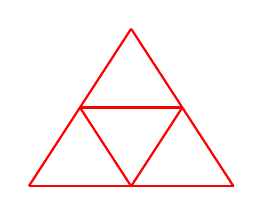
\begin{tikzpicture}
      \draw[color=red, thick] (0, 0)--(1.3, -2);
      \draw[color=red, thick] (0, 0)--(-1.3, -2);
      \draw[color=red, thick] (1.3, -2)--(-1.3, -2);
      \draw[color=red, thick] (0.65, -1)--(-0.65, -1);
      \draw[color=red, thick] (0.65, -1)--(0, -2);
      \draw[color=red, thick] (-0.65, -1)--(0, -2);
    \end{tikzpicture}
  \end{center}
  W każdym z tych trójkątów odległość między dwoma punktami nie może przekraczać $2$. Podzielmy każdy z nich znowu na 4 trójkąty równoboczne o boku długości 1:
  \begin{center}
    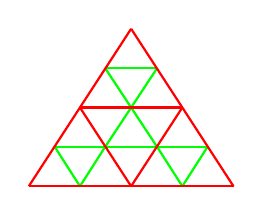
\begin{tikzpicture}
      \draw[color=green, thick] (0.33, -0.5)--(-0.33, -0.5);
      \draw[color=green, thick] (0.33, -0.5)--(0, -1);
      \draw[color=green, thick] (-0.33, -0.5)--(0, -1);
      \draw[color=green, thick] (-0.33, -1.5)--(0, -1);
      \draw[color=green, thick] (0.33, -1.5)--(0, -1);
      \draw[color=green, thick] (-0.97, -1.5)--(0.97, -1.5);
      \draw[color=green, thick] (-0.97, -1.5)--(-0.65, -2);
      \draw[color=green, thick] (-0.33, -1.5)--(-0.65, -2);
      \draw[color=green, thick] (0.97, -1.5)--(0.65, -2);
      \draw[color=green, thick] (0.33, -1.5)--(0.65, -2);
      \draw[color=red, thick] (0, 0)--(1.3, -2);
      \draw[color=red, thick] (0, 0)--(-1.3, -2);
      \draw[color=red, thick] (1.3, -2)--(-1.3, -2);
      \draw[color=red, thick] (0.65, -1)--(-0.65, -1);
      \draw[color=red, thick] (0.65, -1)--(0, -2);
      \draw[color=red, thick] (-0.65, -1)--(0, -2);
    \end{tikzpicture}
  \end{center}
  Dostajemy 16 trójkątów, w środku których odległości nie przekraczają 1. Rozmieszczając 17 punktów mamy pewność, ze co najmniej dwa z nich będą w tym samym trójkącie, więc odległość między nimi nie przekroczy 1.
\newpage
\subsection*{ZAD 13. Na płaszczyźnie danych jest pięć punktów kratowych (o obu współrzędnych całkowitych). Wykazać, że środek jednego z odcinków łączących te punkty też jest kratowy.}
Mamy 2 współrzędne, więc układ parzystych i nieparzystych współrzędnych można wybrać na 4 sposoby.\\
Jest 5 punktów, więc co najmniej dwa z nich mają ten sam układ, więc cih suma będzie miała obie współrzędne parzyste, a więc srodek takiego odcinka ma współrzędne całkowite:
$$x={x_1+x_1\over2}$$
$$y = {y_1+y_2\over2}$$
\newpage
\subsection*{ZAD 18. Na płaszczyźnie danych jest 6 punktów, z których żadne trzy nie są współliniowe. W każdym trójkącei wyznaczonym przez pewna trójkę tych punktów najkrótszy bok malujemy na żółto. Udowodnij, że istnieje trojkat o wszystkich bokach zoltych.}
  Mamy 6 punków, które możemy połączyć w odcinki na
  $${6\choose2}=15$$
  różnych sposobów. Ustawiając je od najdłuższego do najkrótszego, mamy pewność, że dwa najdłuższe nigdy nie będą żółte. Pozostaje nam więc 13 żółtych odcinków.\\
  Rozdzielając 13 odcinków na 6 różnych punktów mamy pewność, ze z pewnego punktu wychodzą co najmniej 3 żółte odcinki. Wiemy, że tylko dwa na pewno będą niepomalowane, a końce tych 3 żółtych odcinków możemy połączyć na 3 sposoby - co najmniej jeden z nich będzie zółty.
  \begin{center}
  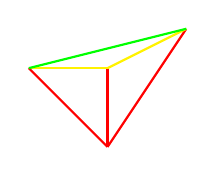
\begin{tikzpicture}
    \draw[red, thick] (0,0) --(1, 1.5);
    \draw[red, thick] (0,0) --(-1, 1);
    \draw[red, thick] (0,0) --(0, 1);
    \draw[yellow, thick] (0, 1)--(-1, 1);
    \draw[yellow, thick](0, 1)--(1,1.5);
    \draw[green, thick](1,1.5)--(-1,1);
  \end{tikzpicture}\end{center}
  \newpage
  \subsection*{ZAD 17. Każdy punkt okręgu pomalowano na jeden z dwóch kolorów. Wykaż, że istnieje trójkąt równoramienny wpisany w ten okrąg, o wszystkich trzech wierzchołkach jednego koloru.}
  Wybierzmy sieczną (niebędącą średnicą) tego okręgu, której oba punkty przecięcia z okręgiem mają ten sam kolor:
  \begin{center}
    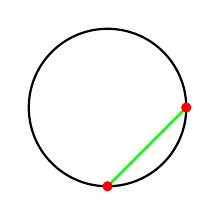
\begin{tikzpicture}
        \draw[thick] (0, 0) circle (1);
        \draw[green, thick] (1, 0)--(0, -1);
        \filldraw[color=red, fill=red, thick] (1, 0) circle (0.05);
        \filldraw[color=red, fill=red, thick] (0, -1) circle (0.05);
    \end{tikzpicture}
\end{center}
    Narysujmy teraz symetralną tej siecznej:
    \begin{center}
        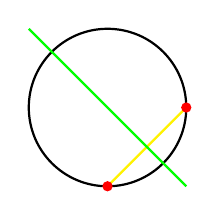
\begin{tikzpicture}
            \draw[thick] (0, 0) circle (1);
            \draw[yellow, thick] (1, 0)--(0, -1);
            \filldraw[color=red, fill=red, thick] (1, 0) circle (0.05);
            \filldraw[color=red, fill=red, thick] (0, -1) circle (0.05);
            \draw[green, thick] (1, -1)--(-1, 1);
        \end{tikzpicture}
    \end{center}
    Jeśli choć jeden punkt przecięcia tej symetralnej z okręgiem jest tego samego koloru, otrzymaliśmy trójkąt równoramienny:
    \begin{center}
        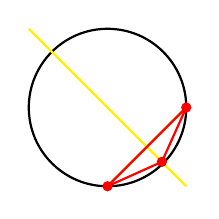
\begin{tikzpicture}
            \draw[thick] (0, 0) circle (1);
            \draw[yellow, thick] (1, 0)--(0, -1);
            \filldraw[color=red, fill=red, thick] (1, 0) circle (0.05);
            \filldraw[color=red, fill=red, thick] (0, -1) circle (0.05);
            \draw[yellow, thick] (1, -1)--(-1, 1);
            \filldraw[color=red, fill=red, thick] (0.69, -0.69) circle (0.05);
            \draw[red, thick] (0.69, -0.69)--(1, 0);
            \draw[red, thick] (0.69, -0.69)--(0, -1);
            \draw[red, thick] (0, -1)--(1, 0);
        \end{tikzpicture}
    \end{center}
    W przeciwnym wypadku rysujemy symetralna tej średnicy:
    \begin{center}
        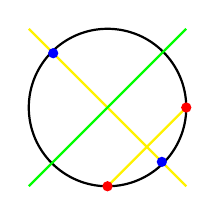
\begin{tikzpicture}
            \draw[thick] (0, 0) circle (1);
            \draw[yellow, thick] (1, 0)--(0, -1);
            \filldraw[color=red, fill=red, thick] (1, 0) circle (0.05);
            \filldraw[color=red, fill=red, thick] (0, -1) circle (0.05);
            \draw[yellow, thick] (1, -1)--(-1, 1);
            \filldraw[color=blue, fill=blue, thick] (0.69, -0.69) circle (0.05);
            \filldraw[color=blue, fill=blue, thick] (-0.69, 0.69) circle (0.05);
            \draw[green, thick] (-1, -1)--(1, 1);
        \end{tikzpicture}
    \end{center}
    Jeśli jeden z jej punktów przecięcia z okręgiem jest niebieski, dostajemy trójkąt rownoramienny:
    \begin{center}
        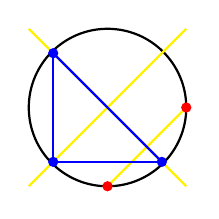
\begin{tikzpicture}
            \draw[thick] (0, 0) circle (1);
            \draw[yellow, thick] (1, 0)--(0, -1);
            \filldraw[color=red, fill=red, thick] (1, 0) circle (0.05);
            \filldraw[color=red, fill=red, thick] (0, -1) circle (0.05);
            \draw[yellow, thick] (1, -1)--(-1, 1);
            \filldraw[color=blue, fill=blue, thick] (0.69, -0.69) circle (0.05);
            \filldraw[color=blue, fill=blue, thick] (-0.69, 0.69) circle (0.05);
            \draw[yellow, thick] (-1, -1)--(1, 1);
            \filldraw[color=blue, fill=blue, thick] (-0.69, -0.69) circle (0.05);
            \draw[blue, thick] (-0.69, -0.69)--(-0.69, 0.69);
            \draw[blue, thick] (-0.69, -0.69)--(0.69, -0.69);
            \draw[blue, thick] (-0.69, 0.69)--(0.69, -0.69);
        \end{tikzpicture}
    \end{center}
    W przeciwnym wypadku dostajemy trapez równoramienny:
    \begin{center}
        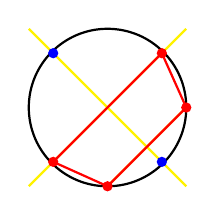
\begin{tikzpicture}
            \draw[thick] (0, 0) circle (1);
            \draw[yellow, thick] (1, 0)--(0, -1);
            \filldraw[color=red, fill=red, thick] (1, 0) circle (0.05);
            \filldraw[color=red, fill=red, thick] (0, -1) circle (0.05);
            \draw[yellow, thick] (1, -1)--(-1, 1);
            \filldraw[color=blue, fill=blue, thick] (0.69, -0.69) circle (0.05);
            \filldraw[color=blue, fill=blue, thick] (-0.69, 0.69) circle (0.05);
            \draw[yellow, thick] (-1, -1)--(1, 1);
            \filldraw[color=red, fill=red, thick] (-0.69, -0.69) circle (0.05);
            \filldraw[color=red, fill=red, thick] (0.69, 0.69) circle (0.05);
            \draw [red, thick] (0.69, 0.69)--(-0.69, -0.69);
            \draw [red, thick] (0.69, 0.69)--(1, 0);
            \draw [red, thick] (-0.69, -0.69)--(0, -1);
            \draw [red, thick] (1, 0)--(0, -1);
        \end{tikzpicture}
    \end{center}
    Narysujmy symetralne jego ramion:
    \begin{center}
        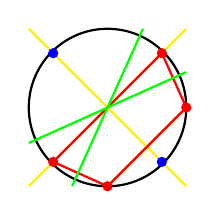
\begin{tikzpicture}
            \draw[thick] (0, 0) circle (1);
            \draw[yellow, thick] (1, 0)--(0, -1);
            \filldraw[color=red, fill=red, thick] (1, 0) circle (0.05);
            \filldraw[color=red, fill=red, thick] (0, -1) circle (0.05);
            \draw[yellow, thick] (1, -1)--(-1, 1);
            \filldraw[color=blue, fill=blue, thick] (0.69, -0.69) circle (0.05);
            \filldraw[color=blue, fill=blue, thick] (-0.69, 0.69) circle (0.05);
            \draw[yellow, thick] (-1, -1)--(1, 1);
            \filldraw[color=red, fill=red, thick] (-0.69, -0.69) circle (0.05);
            \filldraw[color=red, fill=red, thick] (0.69, 0.69) circle (0.05);
            \draw [red, thick] (0.69, 0.69)--(-0.69, -0.69);
            \draw [red, thick] (0.69, 0.69)--(1, 0);
            \draw [red, thick] (-0.69, -0.69)--(0, -1);
            \draw [red, thick] (1, 0)--(0, -1);
            \draw [green, thick] (1, 0.45)--(-1, -0.45);
            \draw [green, thick] (-0.45, -1)--(0.45, 1);
        \end{tikzpicture}
    \end{center}
    Jeśli jedna z nich przecina się w czerwonym punkcie, mamy trójkąt:
    \begin{center}
        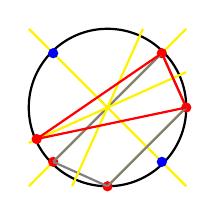
\begin{tikzpicture}
            \draw[thick] (0, 0) circle (1);
            \draw[yellow, thick] (1, 0)--(0, -1);
            \filldraw[color=red, fill=red, thick] (1, 0) circle (0.05);
            \filldraw[color=red, fill=red, thick] (0, -1) circle (0.05);
            \draw[yellow, thick] (1, -1)--(-1, 1);
            \filldraw[color=blue, fill=blue, thick] (0.69, -0.69) circle (0.05);
            \filldraw[color=blue, fill=blue, thick] (-0.69, 0.69) circle (0.05);
            \draw[yellow, thick] (-1, -1)--(1, 1);
            \filldraw[color=red, fill=red, thick] (-0.69, -0.69) circle (0.05);
            \filldraw[color=red, fill=red, thick] (0.69, 0.69) circle (0.05);
            \draw [gray, thick] (0.69, 0.69)--(-0.69, -0.69);
            \draw [gray, thick] (0.69, 0.69)--(1, 0);
            \draw [gray, thick] (-0.69, -0.69)--(0, -1);
            \draw [gray, thick] (1, 0)--(0, -1);
            \draw [yellow, thick] (1, 0.45)--(-1, -0.45);
            \draw [yellow, thick] (-0.45, -1)--(0.45, 1);
            \filldraw[color=red, fill=red, thick] (-0.90, -0.4) circle (0.05);
            \draw[red, thick] (-0.90, -0.4)--(0.69, 0.69);
            \draw[red, thick] (-0.90, -0.4)--(1, 0);
            \draw[red, thick] (1, 0)--(0.69, 0.69);
        \end{tikzpicture}
    \end{center}
    Jeśli żadna nie przecina okręgu w czerwonym pukncie, mamy niebieski trójkąt:
    \begin{center}
        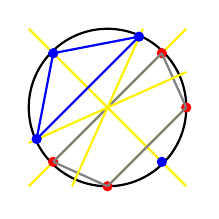
\begin{tikzpicture}
            \draw[thick] (0, 0) circle (1);
            \draw[yellow, thick] (1, 0)--(0, -1);
            \filldraw[color=red, fill=red, thick] (1, 0) circle (0.05);
            \filldraw[color=red, fill=red, thick] (0, -1) circle (0.05);
            \draw[yellow, thick] (1, -1)--(-1, 1);
            \filldraw[color=blue, fill=blue, thick] (0.69, -0.69) circle (0.05);
            \filldraw[color=blue, fill=blue, thick] (-0.69, 0.69) circle (0.05);
            \draw[yellow, thick] (-1, -1)--(1, 1);
            \filldraw[color=red, fill=red, thick] (-0.69, -0.69) circle (0.05);
            \filldraw[color=red, fill=red, thick] (0.69, 0.69) circle (0.05);
            \draw [gray, thick] (0.69, 0.69)--(-0.69, -0.69);
            \draw [gray, thick] (0.69, 0.69)--(1, 0);
            \draw [gray, thick] (-0.69, -0.69)--(0, -1);
            \draw [gray, thick] (1, 0)--(0, -1);
            \draw [yellow, thick] (1, 0.45)--(-1, -0.45);
            \draw [yellow, thick] (-0.45, -1)--(0.45, 1);
            \filldraw[color=blue, fill=blue, thick] (-0.90, -0.4) circle (0.05);
            \filldraw[color=blue, fill=blue, thick] (0.40, 0.9) circle (0.05);
            \draw[blue, thick](0.40, 0.9)--(-0.90, -0.4);
            \draw[blue, thick](0.40, 0.9)--(-0.69, 0.69);
            \draw[blue, thick](-0.69, 0.69)--(-0.90, -0.4);
        \end{tikzpicture}
    \end{center}
\end{document}